
\documentclass[10pt]{beamer}
\usetheme[]{Feather}
\setbeamercolor{Feather}{fg=black!20,bg=black}
\setbeamercolor{structure}{fg=black}
\usepackage[utf8]{inputenc}
\usepackage[spanish]{babel}
\usepackage[T1]{fontenc}
\usepackage{helvet}
\usepackage{lipsum}
\usepackage{amsmath,amssymb,amsfonts}
\usepackage{amsthm}
\usepackage{physics}
\usepackage{framed, color}
\usepackage{epsfig}
\usepackage{acronym}
\usepackage{multirow, array} 
\usepackage{float}
\usepackage[T1]{fontenc}
\usepackage{natbib}
\usepackage{fancyhdr}
\usepackage{xcolor}
\usepackage{multicol}
\usepackage{mdframed}
\usepackage{endnotes}
\usepackage{listings}
\usepackage{tensor}
\usepackage{csquotes}
\usepackage{amsmath}
\usepackage{tikz}
\renewcommand{\thefootnote}{\arabic{footnote}}
\newcommand{\chref}[2]{
  \href{#1}{{\usebeamercolor[bg]{Feather}#2}}
}
\title[]
{
      \textbf{Propuesta de red neuronal DQN para gestión autonóma de tareas en satélites}
}

\subtitle[Propuesta de red neuronal DQN para
gestión autonóma de tareas en satélites]
{Padilla Herrera Carlos Ignacio}

\author[Padilla Herrera Carlos Ignacio]
{      Aprendizaje por refuerzo: DQN
}

\institute[]
{
      }
  
  %there must be an empty line above this line - otherwise some unwanted space is added between the university and the country (I do not know why;( )
}
\date{}
\begin{document}


{\1% % this is the name of the PDF file for the background
\begin{frame}[plain,noframenumbering] % the plain option removes the header from the title page, noframenumbering removes the numbering of this frame only
  \titlepage % call the title page information from above
\end{frame}}
\begin{frame}
  \frametitle{Requisitos de eficiencia energética}
  La red debe garantizar que el estado de carga (SoC) de la batería se mantenga por encima del 20\%, evitando largos periodos por debajo del 30\% para asegurar la longevidad y eficacia del satélite.
\end{frame}

\begin{frame}
  \frametitle{Aprendizaje por refuerzo}
  El aprendizaje por refuerzo o aprendizaje reforzado (en inglés: reinforcement learning) es un área del aprendizaje automático (AA) inspirada en la psicología conductista, cuya ocupación es determinar qué acciones debe escoger un agente de software en un entorno dado con el fin de maximizar alguna noción de \"\ recompensa \"\ o premio acumulado.
\end{frame}


\begin{frame}
  \frametitle{DQN}
  Nuestro modelo será una red neuronal feedforward que toma la diferencia entre los parches de pantalla actuales y anteriores. Tiene dos salidas, representando Q(s, izquierda) y Q(s, derecha) (donde s es la entrada a la red). En efecto, la red intenta predecir la rentabilidad esperada de realizar cada acción dada la entrada actual.
  
  \href{https://pytorch.org/tutorials/intermediate/reinforcement_q_learning.html}{Reinforcement Learning (DQN) Tutorial}
\end{frame}

\begin{frame}
  \frametitle{Capa de entrada}
   El tamaño de esta capa deberá coincidir con el número de entradas que incluyen el SoC de la batería, datos de consumo de tareas, datos de los paneles solares y sensores de luz.
Sumando todas las entradas, tendríamos 1 (SoC) + 10 (tareas) + 15 (paneles solares) + 30 (sensores de luz) = 56 nodos en la capa de entrada.

\end{frame}

\begin{frame}
  \frametitle{Capas ocultas}
  Podemos tener varias capas ocultas, cada una con una cantidad definida de neuronas. Usualmente, estas capas utilizan la función de activación ReLU para introducir no linealidades.
La primera capa oculta podría tener, por ejemplo, 128 nodos, y la segunda capa oculta 64 nodos.

\end{frame}

\begin{frame}
  \frametitle{ReLU}
  En el contexto de las redes neuronales artificiales, la función de activación rectificadora o ReLU (unidad lineal rectificada) es una función de activación definida como la parte positiva de su argumento:

  
  \begin{equation}
  f(x) = \max(0, x)
  \end{equation}


\end{frame}

\begin{frame}
  \frametitle{Capa de salida}
  El tamaño de la capa de salida debe coincidir con el número de acciones posibles. En este caso, cada acción podría representar la decisión de ejecutar una tarea específica o una combinación de ellas.
La capa de salida debe tener tantos nodos como acciones disponibles, cada uno representando el valor Q de tomar esa acción en el estado actual.

\end{frame}

\begin{frame}
  \frametitle{Tabla Q}
\resizebox{\textwidth}{!}{%
\begin{tabular}{c|cccc}
\textbf{Estado / Acción} & \textbf{Ejec. tarea alta pri.} & \textbf{Ejec. tarea baja pri.} & \textbf{Retrasar tarea} & \textbf{Cambiar pri.} \\
\hline
SoC > 30\%, Tareas altas pend. & Q(s_1, a_1) & Q(s_1, a_2) & Q(s_1, a_3) & Q(s_1, a_4) \\
SoC 20-30\%, Tareas altas pend. & Q(s_2, a_1) & Q(s_2, a_2) & Q(s_2, a_3) & Q(s_2, a_4) \\
SoC > 30\%, Tareas bajas pend. & Q(s_3, a_1) & Q(s_3, a_2) & Q(s_3, a_3) & Q(s_3, a_4) \\
SoC 20-30\%, Tareas bajas pend. & Q(s_4, a_1) & Q(s_4, a_2) & Q(s_4, a_3) & Q(s_4, a_4) \\
\end{tabular}%
}




Los estados (s) podrían incluir diversos factores como el estado de carga de la batería (SoC), la lista de tareas pendientes, el consumo actual, entre otros. Las acciones (a) podrían ser:.
\end{frame}

\begin{frame}
  \frametitle{Ecuación de Bellman}
\begin{equation}
V(s) = \max_a \left\{ R(s, a) + \gamma V(s') \right\}
\end{equation}

\end{frame}




\begin{frame}
  \frametitle{Primera versión de implementación}
  \href{https://colab.research.google.com/drive/1Q0qbUixrir5GWn5auAH5yfjDvS-Opwcd?usp=sharing}{Enlace a Google Colab}


  
\end{frame}

\begin{frame}
\frametitle{Arquitectura} % Opcional: puedes poner un título a la diapositiva
\centering % Centrar la imagen en la diapositiva
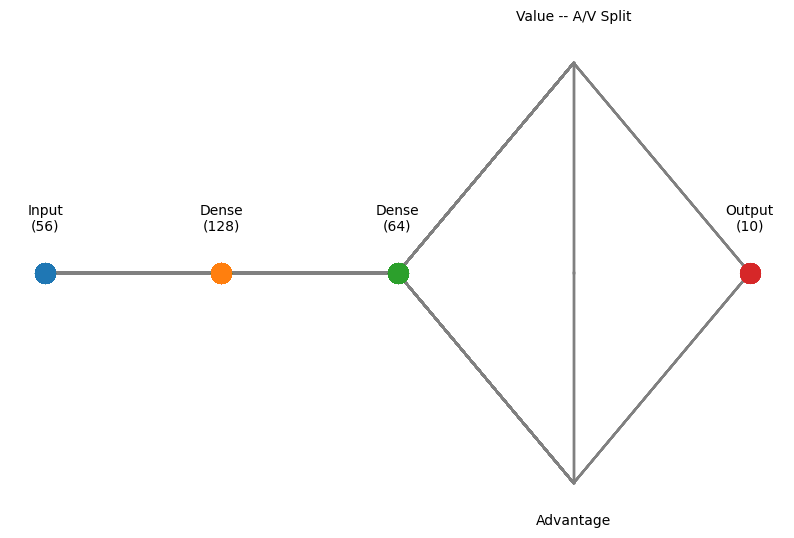
\includegraphics[width=0.8\textwidth]{descarga.png} % Ajusta la ruta y el nombre del archivo
\end{frame}

\begin{frame}
 La red comienza con una capa de entrada de 56 nodos, seguida de dos capas densas con 128 y 64 nodos, respectivamente. Luego se introduce una división para el enfoque Dueling DQN, separando en dos caminos: ventaja y valor, que finalmente se combinan para producir la salida de 10 nodos, representando las acciones posibles. ​
\end{frame}



\end{document}